\documentclass[a4paper, 12pt]{report}

%%%%%%%%%%%%
% Packages %
%%%%%%%%%%%%

\usepackage[english]{babel}
\usepackage[noheader]{packages/sleek}
\usepackage{packages/sleek-title}
\usepackage{packages/sleek-theorems}
\usepackage{packages/sleek-listings}
% \usepackage{algorithmic}
\usepackage{algorithm}
\usepackage{algpseudocode}
\usepackage{multirow}
\usepackage{hyperref}
%%%%%%%%%%%%%%
% Title-page %
%%%%%%%%%%%%%%

\logo{StringMatching.png}
\institute{Habib University}
\faculty{CS 412: Algorithms}
%\department{Department of Anything but Psychology LMAO}
\title{String Matching Problem}
\subtitle{Algorithms to solve it and their analysis}
\author{\textit{Authors}\\Arham Ahmed \\ Maham Shoaib Patel\\ Murtaza Faisal Shafi\\ Khubaib Naeem Kasbati }
%\supervisor{Linus \textsc{Torvalds}}
%\context{Well, I was bored...nice XD}
\date{\today}

%%%%%%%%%%%%%%%%
% Bibliography %
%%%%%%%%%%%%%%%%

\addbibresource{./resources/bib/references.bib}

%%%%%%%%%%
% Others %
%%%%%%%%%%

\lstdefinestyle{latex}{
    language=TeX,
    style=default,
    %%%%%
    commentstyle=\ForestGreen,
    keywordstyle=\TrueBlue,
    stringstyle=\VeronicaPurple,
    emphstyle=\TrueBlue,
    %%%%%
    emph={LaTeX, usepackage, textit, textbf, textsc}
}

\FrameTBStyle{latex}

\def\tbs{\textbackslash}

%%%%%%%%%%%%
% Document %
%%%%%%%%%%%%

\begin{document}
    \maketitle
    \romantableofcontents

    \chapter{Introduction to String Matching Problem}

    The problem of finding occurrence(s) of a pattern string within another string or body of text. There are many different algorithms for efficient searching.\footnote{\hyperlink{https://github.com/murtaza854/CS-412-L1-Project-String-Matching}{You can find all implementations of our algorithms here.}}
    String Matching Problem is simply finding occurrence(s) of a \texttt{pattern} (substring) in a \texttt{text} (string). \\
    Mathematically, the problem is finding occurrence(s) of a \texttt{pattern} $x$ where $x$ is a series of $m$ characters, $x = \langle x_1,x_2,\dots x_m \rangle$, $x_i \in \Sigma, i = 1,2,\dots,m$ in a \texttt{text}, $y$ where $y$ is a series of $n$ characters, $y= \langle y_1,y_2,\dots y_n \rangle, j = 1,2,\dots,n$.\footnote{Definition inspired from CS 369 University of Auckland \cite{Gimelfarb}} 
    \\
    We will be focusing on finding all the occurrences of a \texttt{pattern} in \texttt{text}.
    This problem is relevant in the real world and some of its applications include:
    \begin{enumerate}
        \item Plagiarism detection
        \item DNA sequencing to find patterns of a particular DNA sequence.
        \item Text editors.
        \item Searching for files.
        \item Spam filters.
    \end{enumerate}
    
%     Find one, or more generally, all the occurrences
% of a pattern x = [x0x1..xm−1]; xi ∈ Σ; i = 0, . . . , m − 1, in a text
% (string) y = [y0y1..yn−1]; yj ∈ Σ; j = 0, . . . , n − 1

    % \begin{lstlisting}[style=latexFrameTB, caption={Example of Sleek Template packages usage.}, gobble=8]
    %     \usepackage[english]{babel}
    %     \usepackage[noheader]{packages/sleek}
    %     \usepackage{packages/sleek-title}
    % \end{lstlisting}

    % \blindfootnote{If you are a \LaTeX{} beginner consider the excellent \href{https://www.overleaf.com/learn}{Overleaf tutorial}. Also, there are a lot of symbols available in \LaTeX{} and, therefore, in this template. I recommend the use of \enquote{The Comprehensive \LaTeX{} Symbol List} \cite{pakin2020comprehensive} for searching symbols.}

    \chapter{Solutions to the Problem}
    
    In this portion, we will look at 3 algorithms to solve the string matching problem.
    \begin{enumerate}
        \item Brute Force / Na\"ive Algorithm
        \item Rabin-Karp Algorithm
        \item Knuth-Morris-Pratt Algorithm
    \end{enumerate}
    \section{Brute Force / Na\"ive Algorithm}

    Brute Force or the Na\"ive Algorithm is a relatively easier and simple algorithm to follow. However, the algorithm is slower than other solutions to the problem. It simply creates a window size of size \textit{m} which is equal to the size of the \textit{pattern} being detected in the \textit{text}. It slides the window over every turn and compares the window to the pattern and if it matches then it simply returns a match at the starting index of the window.
    
    Some features of the Brute Force algorithm are as follows:
    \begin{itemize}
        \item It does not require any pre-processing of the text or the pattern.
        \item It shifts the window by 1 after every comparison.
        \item It compares every element in the pattern with every element in the window with no specific order of comparison.
    \end{itemize}

    \subsection{Algorithm}
    The brute force algorithm, as explained above, works through making consecutive comparisons by sliding a window of size \textit{m} (which is the size of the pattern) over a text of size \textit{n}.\\
    After the window is created, we then make comparisons of every letter at index \textit{i} of the window with the letter at same index \textit{i} of the pattern. If every element in the window matches that of the pattern then we return the starting index of the window in the text.
    We can thus write the pseudo code as follows:
    \newpage
        \begin{algorithm}
\begin{algorithmic}
\Procedure{BruteForce}{\texttt{pattern}, \texttt{text}} 
  \For{ $j \gets$ 0 to \texttt{len}(\texttt{text}) $-$ \texttt{len}\texttt{(pattern)} $-\ 1$}
  \For{$i \gets$ 0 to \texttt{len}\texttt{(pattern)} $-\ 1$}
  \If {\texttt{text[i+j]} $\neq$ \texttt{pattern[i]}}
  \State \textbf{break}
  \EndIf
  \If {$i$ = \texttt{len(pattern)} $-\ 1$}

  \State \texttt{print}(i)
  \EndIf
  \EndFor
  \EndFor
  
\EndProcedure
\end{algorithmic}
\end{algorithm}

    \subsection{Example}
    The functionality of the algorithm can be explained by taking the example of the following text: \textbf{ABAACBAABABA} where we need to search for the pattern: \textbf{ABA}. 
    The algorithm will create a window of size \textit{m} which is 3 in this case and create the window over the first three elements of the text as follows:
    \begin{center}
        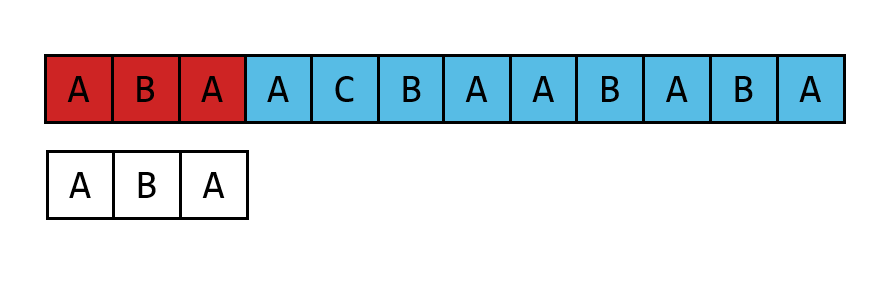
\includegraphics[scale = 0.75]{brute1.PNG}
    \end{center}
    As all the elements of the window and the pattern match, a match is produced at the index of the first element of the window in the text as follows:
    \begin{center}
        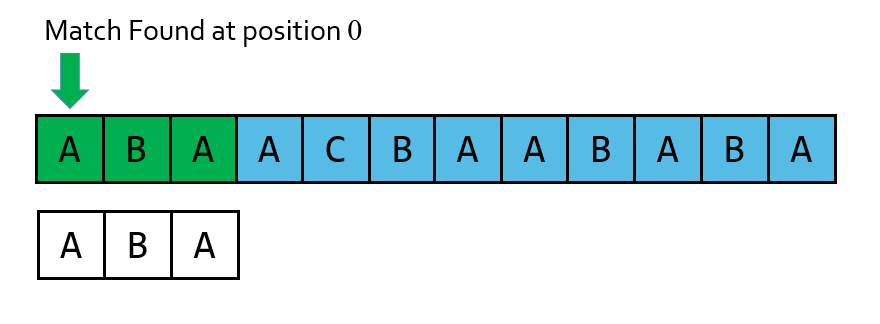
\includegraphics[scale = 0.76]{brute2.PNG}
    \end{center}
    The window then slides over by one and compares all the elements of the window with those of the pattern again. If no match is produced, the window slides to the right by 1 and continues its search. 
    \begin{center}
        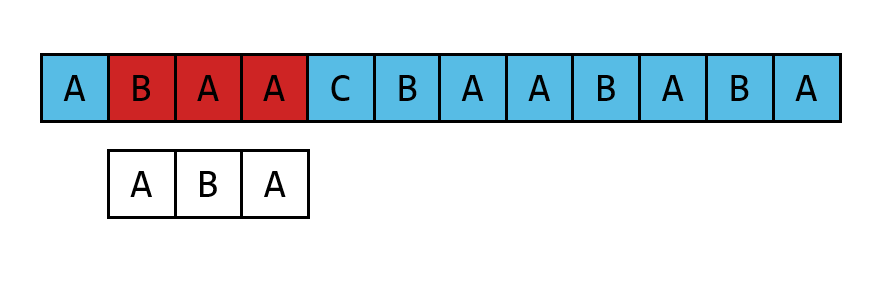
\includegraphics[scale = 0.75]{brute3.PNG}
    \end{center}
    It continues to do so until it reaches the end and prints/returns the indexes of the the first element of the window after every match is produced.

    \subsection{Code}
    The algorithm can be coded in python as follows:
    \FrameTBStyle{python}
    \lstinputlisting[style=pythonFrameTB, gobble=4]{BruteForce.py}
    \subsection{Complexity Analysis}
    The time complexity of the algorithm is $O(n\cdot m)$ as the upper bound for comparisons is $m\cdot n$.



    \newpage
    \section{Rabin-Karp Algorithm}

    Rabin-Karp is an algorithm which tries to avoid unnecessary comparison through hashing, since comparing two hashes is faster than comparing every character one by one. We use a version of hashing called \textbf{rolling hash}.
    \subsection{Rolling Hash}
    A rolling hash is a hash function where the input is hashed in a window which moves across the input. It uses the previously known hash value and the character that enters the window and the one that leaves it in order to compute hash value.
    For that initially, we need to compute the hash value, which can be done using the following algorithm.
    \begin{algorithm}
        \begin{algorithmic}
        \Function{hash}{\texttt{word}, \texttt{quotient}} 
        \State \texttt{result} $\gets 0$
        \State  $m \gets$ \texttt{len(word)}

          \For{$i \gets$ 0 to $m -1$}
          \State \texttt{result} $\gets$ (\texttt{result + ord(word[i])}$\times 2^{m-1-i})  \mod $ \texttt{quotient}
          \EndFor
          \State \Return \texttt{result}
        \EndFunction
        \end{algorithmic}
        \end{algorithm}
        \\
    The Pseudo-code for the rolling hash is as follows
    \begin{algorithm}
        \begin{algorithmic}
        \Function{rollinghash}{\texttt{remove}, \texttt{add}, \texttt{oldvalue}, \texttt{windowsize}, \texttt{quotient}} 
        \State $m \gets $ \texttt{windowsize}
        \State \Return $(2\times$ \texttt{oldvalue} - \texttt{ord(remove)}$\times 2^m+$  \texttt{ord(b)} $)\mod$ \texttt{quotient}
        \EndFunction
        \end{algorithmic}
        \end{algorithm}
    %     def rehash(a, b, hash_text, m, quotient):
    % return (2*hash_text - ord(a)*2**(m) + ord(b))%quotient

    \subsection{Algorithm}

    Let $m$ be size of \texttt{pattern} and $n$ be size of \texttt{text}. The algorithm is as follows:
    \begin{enumerate}
        \item First compute the hash of the first $m$ characters in hash and hash of the \textit{pattern}.
        \item See if the hash of the first $m$ characters matches with the hash of the \textit{pattern}. If so, check the $m$ characters in the window and see if they actually match with the \textit{pattern}. If it does, that is one of our answers.
        \item  Move the window by 1 and calculate the new hash by using the rolling hash function and see if the new hash matches the hash of the \textit{pattern}. If so, check the $m$ characters in the window and see if they actually match with the \textit{pattern}. If it does, that is one of our answers.If the window doesn't end on the last character in the \textit{text}, then repeat this step.
    \end{enumerate}

    The Pseudo-code for the algorithm is as follows:
    \pagebreak
    \begin{algorithm}
        \begin{algorithmic}
        \Procedure{RabinKarp}{\texttt{pattern}, \texttt{text}, \texttt{quotient}} 
        \State $m \gets$ \texttt{len(pattern)}
        \State $n \gets $ \texttt{len(text)}
        \State hashpattern $\gets$ HASH(\texttt{pattern},\texttt{quotient})
        \State hashtext $\gets$ HASH(\texttt{text[:m]},\texttt{quotient})
        \For{$j \gets 0$ to $n-m-1$}
        \If{hashtext = hashpattern \textbf{and} \texttt{text[j:j+m]} = \texttt{pattern}}
        \State \texttt{print(j)}
        \EndIf
        \If{j+m < n}
        \State hashtext $\gets$ ROLLINGHASH(\texttt{text[j]}, \texttt{text[j+m]}, \texttt{hashtext}, m, \texttt{quotient})
        \EndIf
        \EndFor
        
        \EndProcedure
        \end{algorithmic}
        \end{algorithm}  
    
    \subsection{Example}
    The following is the steps taken when the algorithm is given the parameters, \texttt{pattern =} ``CDD'',  \texttt{text =} ``CDDCDD'', \texttt{quotient =} 524287
\begin{verbatim}
text = CDD , hash_text = 472 , hash_word = 472
Pattern is found at position: 0
text = DDC , hash_text = 475 , hash_word = 472
text = DCD , hash_text = 474 , hash_word = 472
text = CDD , hash_text = 472 , hash_word = 472
Pattern is found at position: 3
\end{verbatim}

    \subsection{Code}
    \FrameTBStyle{python}
    \lstinputlisting[style=pythonFrameTB, gobble=4]{RabinKarp.py}
    

    \subsection{Complexity Analysis}

   The Complexity for this algorithm in the worst case is $O(m\cdot n)$ and a case where this can happen is when we have a poor hash function, where the hash function results in a lot of false positives and has to check every pattern like the brute force. But the best/average case is $O(n+m)$ since a lot of character checks are skipped due to hashing.

    \newpage
    \section{Knuth-Morris-Pratt Algorithm }
    KMP algorithm \cite{Knuthf1977} was developed by Knuth Morris and Pratt independently and it is the first ever \textbf{linear time algorithm} for string matching. Unlike brute force, it totally avoids the re-examination of the previously matched characters.

    
    \subsection{Algorithm with an example}

    In order to understand the algorithm, we will first develop it intuitively by working on an example where \texttt{pattern} $=$ \texttt{onions} and \texttt{text} $=$ \texttt{onionions}
    \\
    Every time brute force fails, it starts matching from the next character. In doing this we are not employing the knowledge from our last matching. We can use that knowledge and features of the \textit{pattern} to know where the next matching should begin from or how many characters we can skip.
    These features of the pattern are stored in a prefix table, where for each of the possible string index \(\{1,2,\dots m\}\) ,prefix\([i], i \in \{1,2,\dots m\}\), stores the length of the longest prefix of p which is also a \textbf{proper} suffix of the substring \texttt{pattern[1,\dots, i]}.
    The following is an example of the prefix table.
    \begin{table}[h]
        \centering
        \begin{tabular}{l|l|l|l|l|l|l|}
        \cline{2-7}
        \textit{i}     & 0 & 1 & 2 & 3 & 4 & 5  \\ \hline
        \texttt{pattern[i]} & o & n & i & o & n & s \\ \hline
        \texttt{LPS[i]}     & 0 & 0 & 0 & 1 & 2 & 0 \\ \hline
        \end{tabular}
        \caption{Prefix Table}
        \label{tab:Prefixtable}
        \end{table}  
        \\
    This prefix table can tell us how many characters of the pattern, we don't have to match again if there is a mismatch. \\
    In our example the following happens:
    \begin{enumerate}
        \item The word matches till onion. Then there is a mismatch in the letter between \textbf{i} in the \textit{text} and \textbf{s} in the \textit{pattern}. 
        \item Our LPS array tells us since \textbf{on} is the common prefix and suffix, we can skip the first 2 characters of the \textit{pattern} and try to match the 3rd character of \textit{pattern} with \textbf{i}.
        \item There is a match between 3rd character of \textit{pattern} and \textbf{i} and as we move till the end of the string, there is a match and we find the instance of onions. 
    \end{enumerate}
    
    \subsection{Prefix Table}
    
    we start by taking two pointers, \textit{len} and \textit{i} and set them to $0$ and $1$ respectively and take an array of the size of the pattern and name it \texttt{LPS} for ease. If there is a match at index \textit{len} and index \textit{i}, we will store \textit{len} $+\ 1$ at i'th index of \texttt{LPS} array.
    
    If there is a mismatch and the \textit{len} pointer has not incremented, we will just increment \textit{i} and continue with our search. 
    
    If \textit{len} pointer has incremented and there is a mismatch then we will simply check the value at the index before \textit{len} pointer in the \texttt{LPS} array (\texttt{LPS[len-1])} and assign that value to \textit{len}.

    We will continue this until the $i$ pointer has reached the end.
    
    Here is an example, Consider a string: \\
    \textbf{ABCDABEABF}
    \textit{len} and $i$ are 0. 
    As we can see in the string, character `A' is occurring at $i = 4$, we put \textit{len} $+\ 1$ at \texttt{LPS[i]}, we increment \textit{len} and $i$ then we see `B' after it at $i = 5$, which is matching with the second character of the string so we put $2$ (\textit{len} $+\ 1 = 2$) at \texttt{LPS[i]}. we can observe that `AB' is a suffix which is occurring in the string hence we have accounted that.
    
        \begin{table}[h]
        \centering
        \begin{tabular}{l|l|l|l|l|l|l|l|l|l|l|l}
        \cline{2-11}
        \textit{i}    & 0 & 1 & 2 & 3 & 4 & 5 & 6 & 7 & 8 & 9 \\ \hline
        \texttt{pattern[i]} & \textbf{A} & \textbf{B} & C & D & \textbf{A} & \textbf{B} & E & A & B & F \\ \hline
        \texttt{LPS[i]}     & 0  & 0  &  0 &  0 & 1 & 2 &   &   &   & \\ \hline
        \end{tabular}
        \caption{Prefix Table}
        \label{tab:Prefixtable2}
        \end{table}  
        
    We can see that the character after `B' is not matching with first and second character and we see that \textit{len} pointer has incremented and there is a mismatch, so we will simply check the value at the index before \textit{len} pointer in the \texttt{LPS} array \texttt{(LPS[len-1])} and assign that value to \textit{len}. and continue this strategy until we reach the end.
    

        \begin{table}[h]
        \centering
        \begin{tabular}{l|l|l|l|l|l|l|l|l|l|l|}
        \cline{2-11}
        \textit{i}     & 0 & 1 & 2 & 3 & 4 & 5 & 6 & 7 & 8 & 9\\ \hline
        \texttt{pattern[i]} & A & B & C & D & A & B & E & A & B & F \\ \hline
        \texttt{LPS[i]}     &  0 & 0  & 0 & 0 & 1 & 2 & 0 & 1  & 2  & 0 \\ \hline
        \end{tabular}
        \caption{Prefix Table}
        \label{tab:Prefixtable3}
        \end{table}  
        
    
    \subsection{Pseudocode}
    

The Pseudocode for Knuth Morris Algorithm is as follows:
\newpage
\begin{algorithm}
    \begin{algorithmic}
    \Procedure{KMPSearch}{\texttt{pattern},\texttt{text}}
      \State \texttt{LPS} $\gets $ LPSARRAY(\texttt{pattern})
      \State $i \gets 0$
      \State $j \gets 0$
      \While{ $i < $ \texttt{len(text)}}
      \If{\texttt{text[i]} $=$ \texttt{pattern[j]}}
      \State $i \gets i + 1$
      \State $j \gets j + 1$
      \Else
      \If{j $\neq$ 0}
      \State $j \gets $ \texttt{LPS}[$j-1$]
      \Else
      \State $i \gets i +1$ 
      \EndIf
      \EndIf
      \If{ $j=$ \texttt{len(pattern)}}
      \State \textbf{print}($i-j$)
      \State  $j \gets$ \texttt{LPS}[$j-1$]
      \EndIf
      \EndWhile
    \EndProcedure
    \end{algorithmic}
    \end{algorithm}
    \newpage
    The algorithm to compute the LPS array is as follows:
    \begin{algorithm}
\begin{algorithmic}
\Function{LPSArray}{\texttt{pattern}}
  \State \texttt{prefixlen} $\gets 0$
  \State  $i \gets 1$
  \State \texttt{prefixlen} $\gets 0$
  \State \texttt{LPS} [ \texttt{len(pattern)} ]
  \State \texttt{LPS} $\gets$ [0,\dots,0]
  \While{$i<$ \texttt{len(pattern)}}
  \If{\texttt{pattern[i]} = \texttt{pattern[prefixlen]}}
    \State \texttt{LPS}[$i$] $\gets $ \texttt{prefixlen} $+\ 1$
    \State \texttt{prefixlen} $\gets $ \texttt{prefixlen} $+\ 1$
    \State $i \gets  i+1$
    \Else
    \If{\texttt{prefixlen} $\neq$ 0}
    \State \texttt{prefixlen} $\gets$ \texttt{LPS}[\texttt{prefixlen} $-\ 1$]
    \Else
    \State \texttt{LPS}[$i$] $\gets$ 0
    \State $i \gets i+1$
    \EndIf
\EndIf
  \EndWhile
  \State \Return \texttt{LPS}
\EndFunction
\end{algorithmic}
\end{algorithm}
    \subsection{Code}
    \FrameTBStyle{python}
    \lstinputlisting[style=pythonFrameTB, gobble=4]{Knuth.py}
    
    \subsection{Complexity Analysis}
    Let length of \texttt{pattern} $= m$ and length of \texttt{text} $= n$.The creation of the \texttt{LPS} array takes $O(m)$ time, since i needs to be incremented $O(m)$ times, and the prefixlen change command decreases prefixlen by at least 1, and can be maximum incremented $O(m)$ times in the algorithm hence that statement runs max $O(m)$ times giving complexity $O(m)$
    \\
    The main KMP Algorithm i pointer is incremented $O(n)$ times and j pointer can be rolled back when there are mismatches. Since j can only roll back as much as it has progressed upto mismatch, each character is examined atmost twice, hence there are at most $O(n)$ comparison leading to the algorithm complexity as $O(n+m)$
    \newpage


    \chapter{Empirical Analysis}

    Complexities gives us a fair idea of which algorithm are better in theory. In reality there are other costs as well that hidden in complexity. In complexity analysis, we usually see the worst case, but those are just upper bounds and in reality may not be the same. It also helps compare algorithms with the same complexity, for example Rabin-Karp and Brute Force who have the same worst case analysis.
        \section{Review of Complexities}
        The below are the theoretical complexities that we knew. We can use them to see whether our results match what we would expect or not.
\begin{table}[h]
\centering
\begin{tabular}{|l|l|}
\hline
\textbf{Algorithm}                                          & \textbf{Complexity}       \\ \hline
Brute Force Algorithm                                       & Worst case: $O(nm)$         \\ \hline
\multicolumn{1}{|c|}{\multirow{2}{*}{Rabin-Karp Algorithm}} & Worst case: $O(nm)$         \\ \cline{2-2} 
\multicolumn{1}{|c|}{}                                      & Average/Best Case: $O(n+m)$ \\ \hline
KMP Algorithm                                               & Worst case: $O(n+m)$        \\ \hline
\end{tabular}
\caption{Theoretical Complexities}
\label{tab:Complexities}
\end{table}
    \section{How Analysis was done}
    The analysis was done on the same computer and in the same language (Python) in order to ensure fair comparison.
    \begin{enumerate}
        \item To see the impact of text size, text size was varied from 5000 to 1,000,000 in steps of 5,000
        \item To see the impact of pattern size, pattern size was varied from 100 to 10000 in steps of 50.
        \item In the testing stage, the algorithm was run thrice for each pair of \texttt{(len(text),len(pattern)} done and the average time was taken. This is to account for different CPU loads and to even out the issues.
        \item Printing was disabled so only the time for computation is taken into account.
    \end{enumerate}
    \newpage

    \section{Impact of size of \texttt{text}}
    \begin{figure}[H]
        \centering
        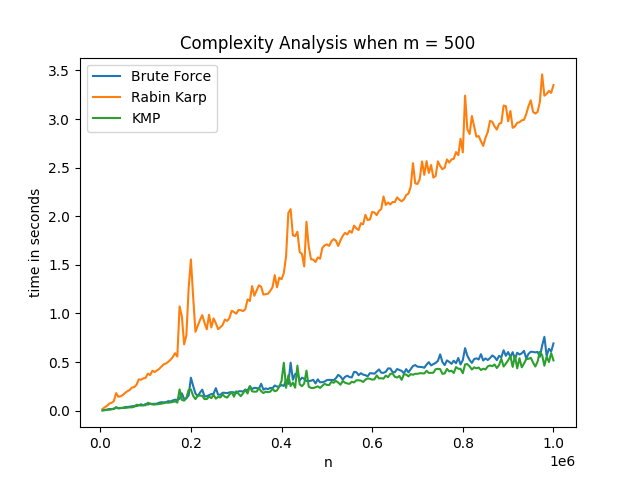
\includegraphics[width=0.8\textwidth]{n_analysis.png}
        \noskipcaption{Analysis increasing size of $n$}
        % \label{fig:random_university_logo}
    \end{figure}
    As size of text increase, time taken increases at a linear rate which is what we expect from complexities since m is fixed. \\
Knuth Morris Pratt Algorithm is taking the least amount of time as we would expect since its complexity is linear and comparisons of a character happen at most 2 times. \\
There is surprising result between Rabin-Karp and Brute Force. Brute Force is much more efficient than Rabin-Karp. The reason for this can be the high cost of hashing which the brute force avoids, there might also be some collisions which result in Rabin-Karp doing more computation in the best case. 
    \section{Impact of size of pattern}
\begin{figure}[H]
        \centering
        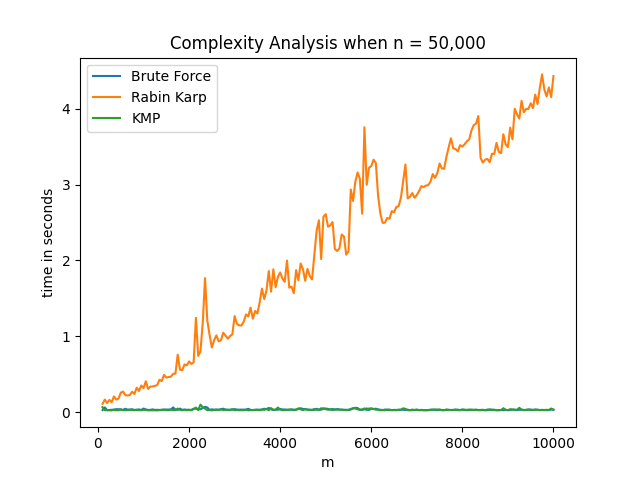
\includegraphics[width=0.8\textwidth]{m_analysis.png}
        \noskipcaption{Analysis increasing size of $m$}
        % \label{fig:random_university_logo}
    \end{figure}
    Knuth Morris Pratt Algorithm takes almost constant as we would expect since $n>m$. Rabin-Karp increases way faster than others. This is because as pattern size increases probability of collisions leading to false positives and hence lot of checking by brute force coupled with cost of hashing, leading to huge growth. Brute force case is strange. This can be because the strings are randomly generated so we don’t have to scan entire string to know it is bad. So worse case isn’t hit.
    
\section{Conclusions}
    KMP Algorithm seems to have the best performance with Brute Force close behind and maybe good for small strings. Rabin-Karp is the slowest but it still is useful, since we can use it to pattern match for multiple patterns at once saving time. The code for evaluation can be found in the repository.
    \printbibliography  
\end{document}
 